\chapter{Analisi del contesto aziendale}
	\section{L'azienda e il suo ambito di attività}
		PastBook è una piccola azienda con sede ad Amsterdam, nei Paesi Bassi. Essa offre agli utenti la possibilità di creare e stampare
		degli album fotografici personalizzati.
		\begin{center}
			
\includegraphics[width=0.4\textwidth]{capitolo_1/immagini/logo_pastbook.png}
		\end{center}
		Il progetto nasce nel 2012 quando Stefano Cutello — fondatore e attuale titolare di PastBook — decide di abbandonare il posto di
		lavoro presso eBay per realizzare la propria idea. L'esigenza è quella di riscoprire i ricordi pubblicati ogni giorno sui social
		network: infatti, le vite delle persone sono ormai completamente online e non esiste più niente di stampato.\\
		L'azienda descrive il servizio che essa offre nel seguente modo:
		\hyphenblockquote{english}{Many things can disappear — not your memories. We believe that certain moments can last forever. We
			believe that the best things in the world are not things. We help you rediscover your memories. We collect the highlights of
			your life moments and provide you with a tangible way to relive them — in PastBook.}
		PastBook, dunque, aiuta le persone a raccogliere le proprie foto sparse per il Web e permette loro di creare un album fotografico
		che memorizzi in modo permanente i ricordi più belli.
	\section{Prodotti offerti}
		\subsection{Photo Books in un click}
			Esistono varie aziende che permettono agli utenti di creare album fotografici a partire dalle immagini presenti nei social
			network. PastBook differisce da esse per un importante principio che sta alla base della realizzazione del prodotto: l'utente
			deve poter creare il proprio Photo Book in modo veloce ed automatico, senza pensare a particolari che distolgano la sua mente
			dallo scopo.\\
			L'azienda prevede che i propri clienti debbano solo scegliere il servizio dal quale intendono ottenere le immagini. Il resto
			è automatico: non è previsto che l'utente abbia la possibilità di personalizzare il proprio Photo Book durante la sua
			realizzazione. I più esigenti possono fare piccole modifiche solo a creazione avvenuta.\\
			\begin{multicols}{3}[\noindent PastBook permette di recuperare le immagini utilizzando uno dei seguenti servizi Web:]
				\begin{itemize}
					\item Instagram
					\item Facebook
					\item Flickr
					\item Google Drive
					\item Dropbox
					\item OneDrive
					\item Picasa
					\item Evernote
					\item Box
				\end{itemize}
			\end{multicols}
			\begin{center}
				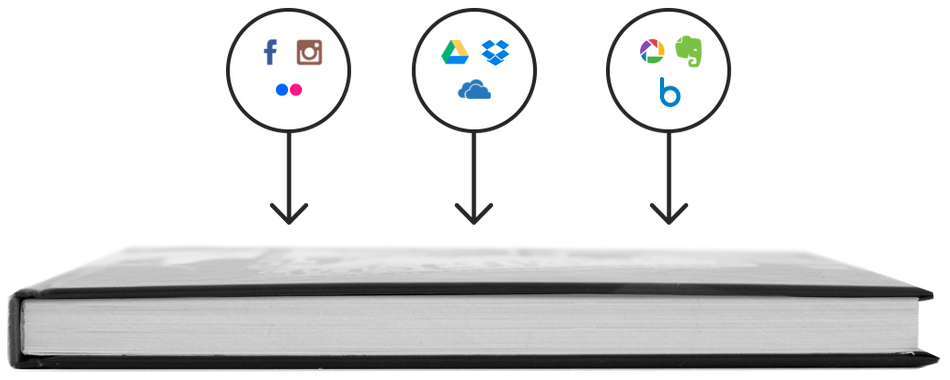
\includegraphics[width=0.9\textwidth]{capitolo_1/immagini/photo_book_one_click.png}
			\end{center}
			Gli utenti hanno inoltre la possibilità di invitare chiunque ad aggiungere ulteriori ricordi al proprio Photo Book,
			condividendo un link privato tramite email, QR code, Facebook o Twitter.
